
% Inbuilt themes in beamer
\documentclass{beamer}

% Theme choice:
%\usetheme{CambridgeUS}

\usepackage{graphicx} % Allows including images

% Title page details: 
\title{Mid-Term Presentation} 
\author{Group A}
\date{\today}
\logo{\large \LaTeX{}}


\begin{document}

% Title page frame
\begin{frame}
    \titlepage 
\end{frame}

% Remove logo from the next slides
\logo{}

%--BISHESH 
	
\begin{frame}{Introduction}
	\begin{itemize}
		\item  Finite Element Method (FEM) is a procedure of numerical solution of a domain viewed as the collection of sub-domains.
		\vspace{0.6cm}
		\item FEM on static structures computing the stress and displacement.
		\vspace{0.6cm}
		\item The actual problem will be replaced by simpler ones to find one approximate solution. 
	\end{itemize}
	
\end{frame}


\begin{frame}{Gantt Chart : Progress}
	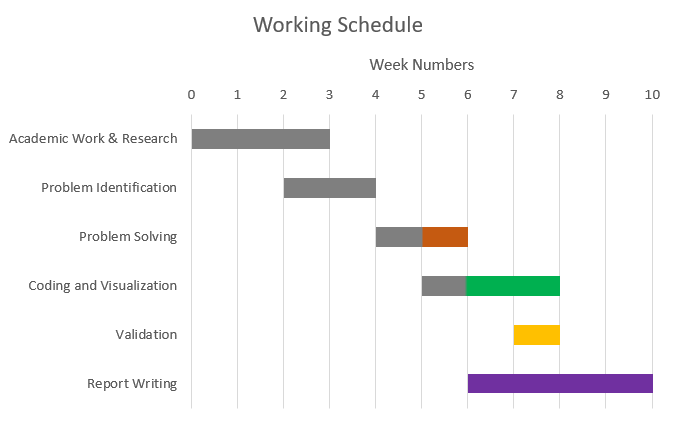
\includegraphics[width = 10cm, height = 6cm]{progress.png}
\end{frame}

%---PRIYANKA

\section{{PROGRESS}}
\begin{frame}[t]{\textbf{\huge{Progress so far...}}}\vspace{20pt}
	\begin{block} {\textbf{\color{black}{\large{Theoritical Background}}}}
		Studied about FEM and its applications
	\end{block}  \vspace{20pt}
	
	\begin{block} {\textbf{\color{black}{\large{Probem solving and identification}}}}
		solved various problems manually and  continued working on truss.
	\end{block}  \vspace{20pt}
	\begin{alertblock}{\textbf{\color{black}{\large{Implementation And Analysis}}}}
		implemented in python in multiple attempts  and analyzed. 
	\end{alertblock}  \vspace{20pt}
\end{frame}


\begin{frame}
	\begin{exampleblock}{\textbf{\color{black}{\large{Class Implementation}}}}
		custom classs in jupyter notebook for nodes and matrices.
		
		
	\end{exampleblock}\vspace{20pt}
	
	
	
	\begin{block} {\textbf{\color{black}{\large{Mechanical Approach}}}}
		followed joint and sectional method and verified .
	\end{block}\vspace{20pt}
	
	\begin{block}{\textbf{\color{black}{\large {Visualization}}}}
		code for visualizing any problem given the coordinates.
		
	\end{block}
	
\end{frame} 

%---SAMRAJYA

% Lists frame
\section{Things left}
\begin{frame}{Things left}
	
	Working of solution:
	\begin{itemize}
		\item Solution part is working for some problem but not for all.
		\item Why, how and in which cases the solution can work in all problem is to be worked on.
		
	\end{itemize}
	
	Software Visualization:
	\begin{itemize}
		\item Data has been generated, solved upon and visualized to an extent both theoretically and manually.
		\item The streamlining of all these components and compiling it is needed.
		
	\end{itemize}
	
\end{frame}

% Lists frame
\section{Things left}
\begin{frame}{Things left}
	
	Theoretical readings:
	\begin{itemize}
		\item As of now, we have only worked and implemented on software.
		\item Knowledge of mandatory principles and applications of FEM is to be thoroughly studied.
		
	\end{itemize}
	
	Report Writing:
	\begin{itemize}
		\item Final report of the project is to be written.
		
		
	\end{itemize}
	
\end{frame}


\end{document}
